\chapter{Costraint Satisfaction Problems} \label{ch:Costraint Satisfaction Problems}
\section{Costraint Satisfaction Problems}
Un vincolo è semplicemente una relazione logica tra diverse incognite (o variabili), ognuna delle quali assume un valore in un dato dominio. Un vincolo quindi restringe i possibili valori che le variabili possono assumere ne rappresenta alcune informazioni parziali sulle variabili di interesse. 
\vspace{0.5cm}
\\Un CSP o \textbf{Problema di Soddisfacimento di Vincoli} formalmente è una tripla:
\begin{center}
    $(X, D, C)$
\end{center}
\begin{itemize}
    \item X è un insieme finito di \textbf{variabili} $\{x_1, ..., x_n\}$
    \item D è una funzione che associa ad ogni variabile un insieme di valori chiamato dominio, cioè tutti i valori che una variabile può assumere.
    \item C è un \textbf{insieme di vincoli}  $\{c_1, ..., c_n\}$ che delimitano le combinazioni di valori ammissibili per la soluzione del problema. 
    \\Possono essere descritti in maniera:
    \begin{itemize}
        \item $Intenzionale:$ Specifico tutte le tuple che sono permesse (WA $\neq$ NT)
        \item $Estenzionale:$ Utilizzando altre funzioni o predicati, tipo $X_1 = 2X_2$ oppure (WA, NT) $\in$ $\{(red, green), ...\}$.
    \end{itemize}
\end{itemize}
\newpage
Ogni vincolo $C_i$ coinvolge alcuni sottoinsiemi di variabili e specifica le combinazioni di valori consentite per quel sottoinsieme. Uno \textbf{stato del problema} è definito da \textbf{un’assegnazione di valori} ad alcune o a tutte le variabili $\{X_i=v_i, X_j=vj, ... \}$. Un’assegnazione che non viola alcun vincolo è chiamata assegnazione \textbf{coerente o legale}. \textbf{Un’assegnazione completa} è quella in cui viene menzionata ogni variabile, e una \textbf{soluzione} a un CSP è un’assegnazione completa che soddisfa tutti i vincoli. Alcuni CSP richiedono anche una soluzione che massimizzi una \textbf{funzione obiettivo}. Ciascun vincolo limita la combinazione di valori che un insieme di variabili può assumere contemporaneamente. Una soluzione di un CSP è l’assegnazione a ciascuna variabile di un valore dal suo dominio che soddisfi tutti i vincoli. Il compito è trovare una soluzione o tutte le soluzioni. Pertanto, il CSP è un problema combinatorio che può essere risolto mediante la ricerca.
\vspace{0.5cm}
\\Per comprendere meglio un problema di soddisfacimento di vincoli è opportuno evidenziare i concetti di stato e di assegnamento:
\begin{itemize}
    \item \textbf{Stato:} Rappresenta ogni combinazione di valori assunti dalle variabili $\{x1,..., xn\}$.
    \item \textbf{Assegnamento:} Rappresenta la soluzione del problema, cioè assegnare dei valori a tutte le variabili (assegnamento completo) in modo tale da soddisfare tutti i vincoli del problema (”assegnamento consistente”).
\end{itemize}
\begin{enumerate}
    \item Un assegnamento è \textbf{inconsistente} se viola un vincolo.
    \item Un CSP è \textbf{soddisfacibile} se esiste almeno una soluzione.
    \item Un assegnamento a un sottoinsieme S delle variabili è localmente consistente se soddisfa i vincoli esistenti tra le variabili in S.
\end{enumerate}
\subsection{Constraint Solving}
La risoluzione dei vincoli differisce dalla soddisfazione dei vincoli poiché utilizza variabili con domini infiniti come i numeri reali. Inoltre, i singoli vincoli sono più complicati, ad esempio non lineari, uguaglianze...
\newpage
\subsection{Esempi}
\subsubsection{Esempio 1}
\textbf{Problema:} Assegnazione delle ore di lezione dei professori (Time Tabling).

\vspace{0.2cm}

\textbf{Dato}: ”Il prof A non può fare lezione dalle 11 alle 13”, ” Il prof B non può fare lezione nell’Aula B” che sarebbero i vincoli, l’obiettivo è avere un assegnamento per tutte le variabili del problema (che saranno i professori e le aule).

\vspace{0.2cm}

Il CSP quindi è un modo di rappresentare i problemi attraverso una serie di relazioni.
\subsubsection{Esempio 2}
Lavoriamo in una mappa dell’Australia che mostra ciascuno dei suoi stati e territori e il compito ci viene affidato è di colorare ogni regione di rosso, verde o blu in modo tale che le regioni vicine non hanno lo stesso colore. Per formulare questo come un CSP, definiamo le variabili come le regioni: WA, NT, Q, NSW , V , SA e T. Il dominio di ciascuna variabile è l’insieme $\{rosso, verde, blu\}$. I vincoli richiedono che le regioni vicine abbiano colori distinti; ad esempio, le combinazioni consentite per WA e NT sono le coppie
\begin{center}
    $\{(rosso, verde), (rosso, blu), (verde, rosso), (verde, blu), (blu, rosso), (blu, verde)\}$ 
\end{center}
Ci sono molte soluzioni possibili, come \{W A = rosso, AN D = verde, A = rosso, N SW = verde, V = rosso, SA = blu, T = rosso\}. 
\\È utile visualizzare un CSP come grafico di vincoli. I nodi del grafico corrispondono a variabili del problema e gli archi corrispondono a vincoli
\begin{figure}[htp]
	\centering
    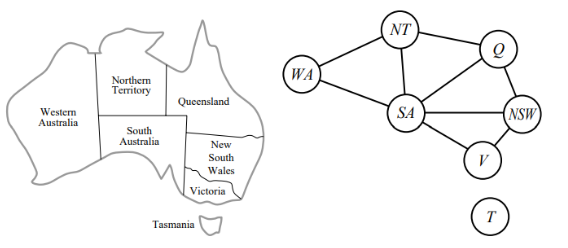
\includegraphics[width=10cm, keepaspectratio]{img/Cap1/map-coloring1.png}
    \caption{Map-Colouring}
\end{figure}
\newpage
\begin{figure}[htp]
	\centering
    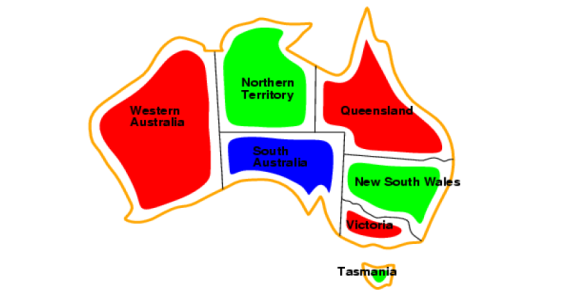
\includegraphics[width=10cm, keepaspectratio]{img/Cap1/map-coloring2.png}
    \caption{Soluzione Map-Colouring}
\end{figure}
In un CSP binario ogni vincolo è in relazione con due variabile. Il tipo più semplice di CSP coinvolge variabili che sono discrete e hanno domini finiti, i problemi di colorazione della mappa sono di questo tipo.
\subsection{Tipi di CSP}
I CSP si suddividono in base ai tipi delle variabili e dei vincoli:
\subsection{Tipi di Variabili}
Le variabili \textbf{discrete} possono avere domini:
\begin{itemize}
    \item \textbf{Finiti:} grandezza dell’assegnamento completo $d \rightarrow O(d^n)$;
    \item \textbf{Infinti:} 
    \begin{itemize}
        \item hanno bisogno di un linguaggio di vincoli
        \item i vincoli lineari sono risolvibili, i non lineari sono indecidibili;
    \end{itemize}
\end{itemize}
Le variabili \textbf{continue}:
\begin{itemize}
    \item Tempo di inizio e fine per specifici problemi (Hubble telescope)
\end{itemize}
Le variabili continue con dei vincoli lineari sono risolvibili in un tempo polinomiale
dai metodi LP.
\newpage
\subsection{Tipi di vincoli}
\begin{itemize}
    \item \textbf{Unari:} I vincoli coinvolgono una singola variabile. $SA \neq green$
    \item \textbf{Binari:} I vincoli coinvolgono coppie di variabili. SA $\neq$ W A
    \item \textbf{High order:} I vincoli coinvolgono tre o più variabili.
    \item \textbf{Preferences:} Ho una preferenza su un valore piuttosto che un altro per una certa variabile. Questi sono anche chiamati vincoli Soft, che rappresentano un costo per ogni $assegnamento$ di variabile.
\end{itemize}
Inoltre i vincoli possono essere espressi in maniera:
\begin{itemize}
    \item \textbf{Implicita:} non viene direttamente indicata la relazione fra gli elementi del dominio che sono permessi. Un esempio può essere x<y, dove non si elencano tutti i possibili assegnamenti delle variabili che non violano quel vincolo ma si possono calcolare;
    \item \textbf{Esplicita:} si elencano tutti i valori ammessi per le variabili coinvolte nel vincolo. 
\end{itemize}
Nell’esempio precedente si avranno tutte le coppie di valori ammessi in base a quel
vincolo.
\newpage
\subsection{Caratteristiche e Propietà CSP}
\begin{enumerate}
    \item \textbf{Commutatività:} Si considera l’assegnamento di una singola variabile per volta.
    \item \textbf{Monotonicità:} Appena un vincolo viene violato posso interrompere la ricerca perchè sono sicuro che non esisterà soluzione.
    \item \textbf{L’ordine} con il quale seleziono le variabili e assegno i valori è molto importante, abbiamo bisogno di euristiche intelligenti.
    \item \textbf{Indipendenza:} quando le variabili non hanno vincoli tra di loro (come ad esempio sulla mappa dell’Australia c’era la T che non era collegata agli altri nodi), il problema si può decomporre in sotto problemi che possono essere risolti in modo indipendente.
    \item É applicabile un controllo per \textbf{consistenza:} Invece di fare un controllo di consistenza alla fine, lo faccio ad ogni passo.
    \item Caso speciale di un problema di ricerca
    \item I domini possono essere discreti o continui
\end{enumerate}
\subsection{Standard search formulation}
Gli stati sono definiti dal valore assegnato finora:
\begin{itemize}
    \item \textbf{Stato iniziale: }assegnamento vuoto \{\};
    \item \textbf{Funzione successore: }assegna un valore a una variabile non assegnata che non va in conflitto con l’assegnamento corrente;
    \item \textbf{Goal test: }l’assegnamento corrente è completo. Questa formula viene usata per tutti i CSP e ogni soluzione appare a profondità n con n variabili. Il cammino è irrilevante, così che può usare la formulazione complete-state.
\end{itemize}

